
\section{Results and Analysis}
\subsection{1-Site Model}
The 1-Site model is the simplest version of the Hubbard-Model as it requires no hopping term and has only 4 states and can be compared to the exact results.
\subsubsection{Comparison $N$ and $N_t$}
\begin{figure}[H]
	\centering
	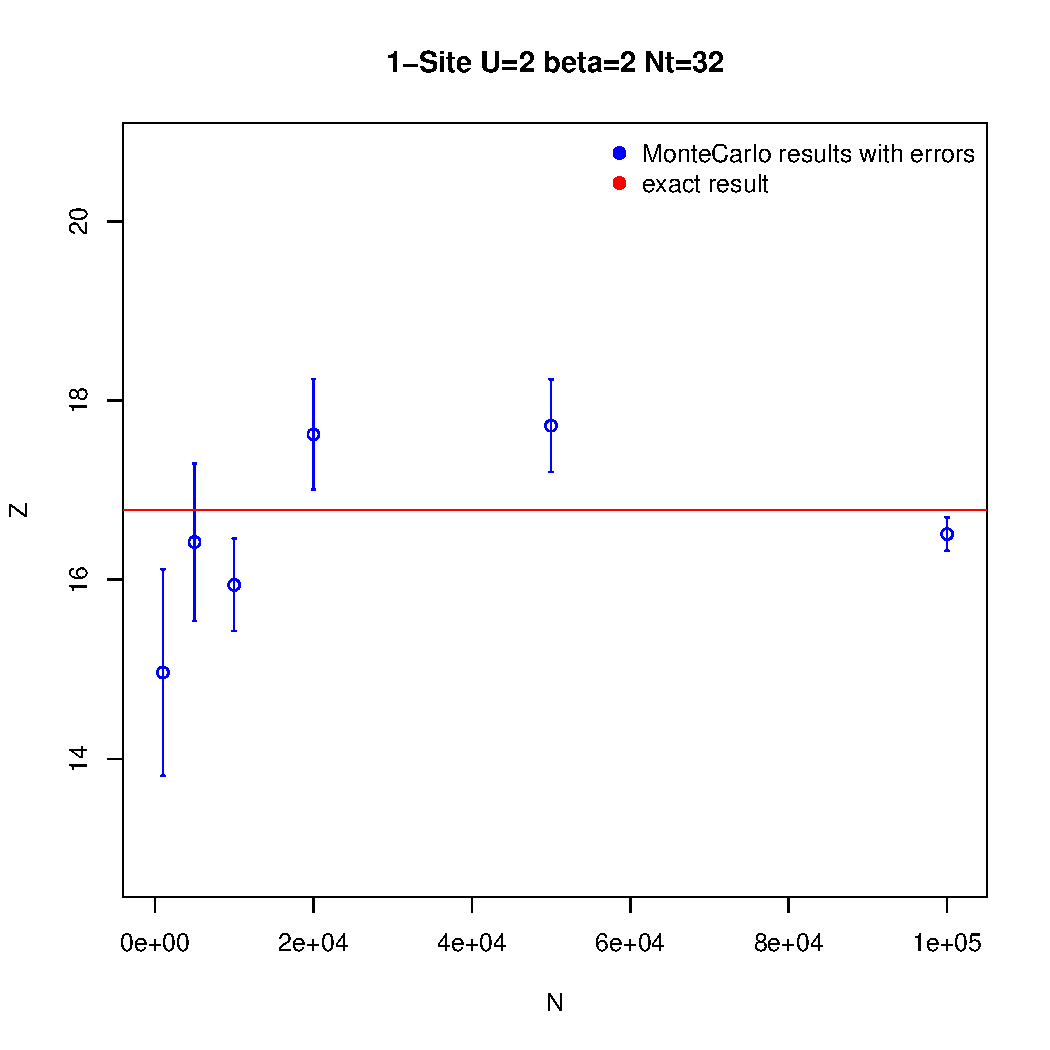
\includegraphics[width=0.7\linewidth]{figs/plot_Z1N}
	\caption[Scaling of Z with N]{This plot shows the result of Z with $U=2$, $\beta=2$ and $N_t=32$ for different numbers of samples.}
	\label{fig:plotz1n}
\end{figure}
Figure \ref{fig:plotz1n} shows how the result depends on the number of samples we average over. While the true accuracy gets slightly better it is clear that the calculated bootstrap error, which gives the statistical error of the Monte-Carlo calculation, becomes smaller for more samples, as expected. The reason why our results are not more accurate is the systematical error from the Hubbard-Stratanovich/ Pathintegral approximation. This one can be improved by increasing the number of timeslices $N_t$.
\begin{figure}[H]
	\centering
	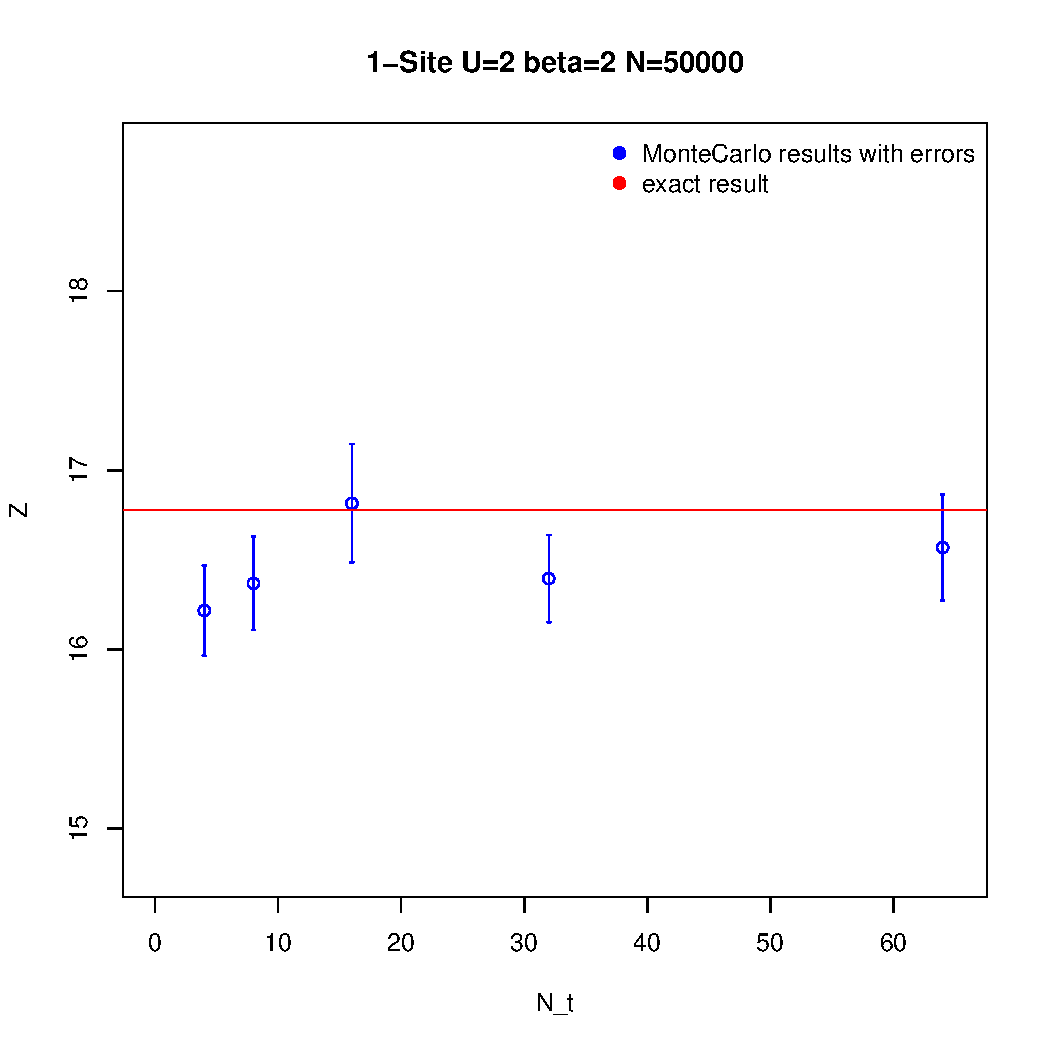
\includegraphics[width=0.7\linewidth]{figs/plot_Z1Nt}
	\caption[Scaling of Z with N_t]{This plot shows the result of Z with $U=2$, $\beta=2$ and $N=50000$ for different numbers of time steps.}
	\label{fig:plotz1nt}
\end{figure}
In figure \ref{fig:plotz1nt} we see the scaling of the result with the number of time slices. This time the statistical error is almost identical for all measurements, while the results slightly come closer to the exact result. This will be clearer for lattices with hopping terms.